\documentclass[aspectratio=169, 12pt]{beamer}
\usepackage{bbm}
\usepackage[utf8]{inputenc}
\usepackage[T2A]{fontenc}
\usepackage[english]{babel}
\usepackage{amscd,amssymb}
\usepackage{amsfonts,amsmath,array}
\usepackage{sidecap}
\usepackage[T2A]{fontenc}
\usepackage[utf8]{inputenc}
\usepackage{graphicx}				% Вставка картинок правильная
\graphicspath{{pictures/}, {images/}, {}}
\DeclareGraphicsExtensions{.pdf,.png,.jpg}
\usepackage{pdfpages}
\usepackage{multicol}

% Для алгоритмов
\usepackage{amsmath}
\usepackage{amsthm}
\usepackage{amssymb}
\usepackage{mathtools}
\usepackage{algorithm}
\usepackage{algpseudocode}
% Цвета 
\usepackage{color}
\usepackage{colortbl}
% Создаем новую команду для assumptions
%----------------------------------------------------------------------------------------------------------

\newtheorem{assumption}{Assumption}
%beamer  theme's used to be here :)
%\usetheme{mipt_beamer}
\usetheme{boxes}

%----------------------------------------------------------------------------------------------------------
\title[\hbox to 56mm{Feature}]{Copulas, Sklar’s Theorem, and Distributional
Transform}
\author[M.\,K.~Kreinin]{Matvei Kreinin, BSc.}
\institute{Moscow Institute of Physics and Technology}
\date{\today}

\begin{document}
\maketitle

\begin{frame}{Table of contents}
    \tableofcontents
\end{frame}

\section{Motivation}
\begin{frame}{Motivation}
\begin{center}
    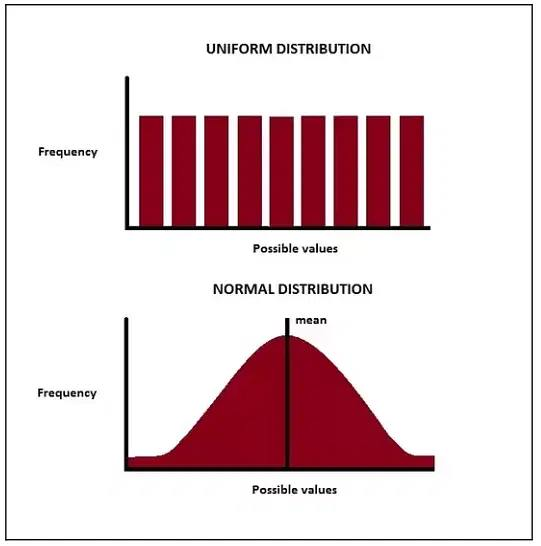
\includegraphics[scale=0.4]{2024-09-23 23.24.49.jpg}
\end{center}
\end{frame}


\section{Problem statement}
\begin{frame}{Problem statement}
    \begin{definition}
        Consider a random vector $(X_1, X_2, ..., X_d)$. Suppose its marginals are continuous, i.e. the marginal CDFs $F_i(x) = \mathbb{P}(X_i \leq x) $ are continuous functions. By applying the probability integral transform to each component, the random vector
        $$
        (U_1, U_2, ..., U_d) = (F_1(X_1), F_2(X_2), ..., F_d(X_d)) 
        $$ has the marginals thar are uniformly distributed on the interval $[0, 1]$.
        The copula of $(X_1, X_2, ..., X_d)$ is defined at the join cumulative distribution function of $(U_1, U_2, ..., U_d)$:
        $$
        C(u_1, u_2, ..., u_d) = \mathbb{P}(U_1 \leq u_1, U_2 \leq u_2, ..., U_d \leq u_d)
        $$
    \end{definition}
\end{frame}

\begin{frame}{Problem statement}
    \begin{definition}
      The reverse of these steps can be used to generate pseudo-random samples from general classes of multivariate probability distributions. That is, given a procedure to generate a sample 
      $$
      (X_1, X_2, ..., X_d) = (F_1^{-1}(U_1), F_2^{-1}(U_2), ..., F_d^{-1}(U_d))
      $$
      The generalized inverses $F_i^{-1}$ are unproblematic almost surely, since the $F_i$ were assumed to be continuous. Furthermore, the above formula for the copula function can be rewritten as:
      $$
      C(u_1, u_2, ..., u_d) = \mathbb{P}(X_1 \leq F_1^{-1}(u_1), X_2 \leq F_2^{-1}(u_2), ..., X_d \leq F_d^{-1}(u_d))
      $$
    \end{definition}
\end{frame}


\section{Theory}
\begin{frame}{Theorem}
\begin{definition}
        In probabilistic terms, $C: [0, 1]^d \rightarrow [0, 1]$ is a d-dimensional copula if C is a joint cumulative distribution function of a d-dimensional random vector on the unit cube $[0, 1]^{d}$ with uniform marginals.
\end{definition}
 \begin{theorem}
 Let $F \in \mathcal{F} (F_1, ..., F_n)$ be an $n-$dimensional distribution function with marginals $F_1, ..., F_n$. Then there exists a copula $C \in \mathcal{F}(\mathcal{U}, ..., \mathcal{U})$ with uniforms marginals such that
 $$
 F(x_1, ..., x_n) = C(F_1(x_1), ..., F_n(x_n))
 $$
 \end{theorem}
\end{frame}


\section{Applications}
\begin{frame}{Applications}
\begin{itemize}
    \item Generative Models and Variational Autoencoders (VAEs)
    Traditional VAEs typically assume independent latent variables with Gaussian priors. By applying copulas based on Sklar’s Theorem, more complex dependencies among latent variables can be captured, allowing for more flexible and realistic data generation.
    \item Time Series Modeling and Sequential Data (Financial, Weather, IoT)
    In time series analysis, especially in applications like finance or weather forecasting, the relationship between variables can exhibit complex dependencies beyond what can be captured using simple correlation. Copulas can capture tail dependencies and non-linear relationships between variables, making them valuable for multivariate time series prediction.
\end{itemize}
    
\end{frame}
\begin{frame}{Links}
    \begin{itemize}
        \item Deriving the joint probability of default of two entities with the Gaussian Copula, \href{https://library .wbi.ac.id/repository/64.pdf}{book}, p. 77
        \item Copulas, Sklar’s Theorem, and Distributional Transform, \href{https://link.springer.com/chapter/10.1007/978-3-642-33590-7_1}{article}
        \item \href{https://www.youtube.com/playlist?list=PLJYjjnnccKYDppALiJlHskU8md904FXgd}{Copula Short Course}
    \end{itemize}
    
    
    
    
\end{frame}
    

\end{document}